\documentclass{rvcepaper}
\newcommand{\orrow}{\multicolumn{6}{|c|}{\bfseries OR}\\ \hline}
\newcommand{\instrA}[1]{\begin{seeinstr}\item Answer all questions from Part A. Part A questions should be answered in first three pages of the answer book only.\item Answer FIVE full questions from Part B. In Part B question number 2 is compulsory. Answer any one full question from 3 and 4, 5 and 6, 7 and 8, 9 and 10.#1\end{seeinstr}}
\begin{document}

%%%%%%%%%%%%%%%%%%%%%%%%%%%%%%%%%%%%%%%% ELEMENTS OF FINANCIAL MANAGEMENT
% ---------------- 21IE6F8, Sept/Oct 2024
\begin{seepaper}
\paperinfo{code={21IE6F8},examline={VI Semester B.E. Regular Examinations Sept/Oct -- 2024},dept={},title={ELEMENTS OF FINANCIAL MANAGEMENT (ELECTIVE)},time={03 Hours},maxmarks={100}}
\seehead
\instrA{\item Usage of interest factor tables is permitted.}
\seepartA
\begin{seeA}
\qaq{1}{1.1}{List the three broad areas of financial decision making.}{02}{01}{01}
\qa{1.2}{What is the primary function of a financial intermediary in Indian financial system?}{02}{02}{01}
\qa{1.3}{What is the meaning of ``perpetuity'' in the context of Time value of money?}{02}{02}{01}
\qa{1.4}{Distinguish between the terms, ``Market Risk'' and ``Unique Risk''.}{02}{02}{01}
\qa{1.5}{List the 3 distinct features of capital expenditure.}{02}{01}{02}
\qa{1.6}{What is meant by the term, ``Cost of retained earnings''?}{02}{02}{02}
\qa{1.7}{Distinguish between `primary Market' and `Secondary market'.}{02}{02}{03}
\qa{1.8}{Distinguish between `Initial Public Offer' and `Follow on public offer'.}{02}{02}{03}
\qa{1.9}{Distinguish between the terms -- Absorption and Consolidation in the context of Mergers.}{02}{02}{04}
\qa{1.10}{Distinguish between the terms -- call option and put option.}{02}{02}{04}
\end{seeA}
\seepart{PART-B}
\begin{seeB}
\qb{2}{a}{What is meant by a financial market? Summarize the categorization of financial markets based on several criterion.}{08}{03}{01}
 & b & List any four types of financial intermediaries prevalent in India. Evaluate the benefits of having financial intermediaries in the financial system. & 08 & 03 & 01\\ \hline
\qb{3}{a}{An amount of $Rs\,1000/-$ is annually deposited for 5 years and the deposit earns a compound interest rate of 10\%. What will be the value at the end of 5 years? Assuming that each deposit occurs at the end of the year, determine the future of annuity.}{05}{03}{01}
 & b & Your friend promises to give you $Rs.\,1000/-$ 6 years later. What is the present value of this amount if the interest rate is 10\%? & 05 & 03 & 01\\
 & c & An investor expects to receive the following cash flows from an asset.
\qtabc{|c|c|c|c|}{\hline \textit{Year} & 1 & 2 & 3\\\hline \textit{Cash Flow (Lakhs in rupees)} & 20 & 30 & 220\\\hline}
The discount rate for cash flows is 16\%. Determine the value of the Asset. & 06 & 03 & 01\\ \hline
\orrow
\qb{4}{a}{A $Rs\,1000/-$ par value bond, bearing a coupon rate of 14\% will mature after 5 years. The required rate of return on this bond is 13\%. What is the value of Bond?}{05}{03}{01}
 & b & An equity share is expected to provide a dividend of $Rs\,2/-$ and fetch a price of $Rs\,18/-$ a year hence. What price would it sell for now if investors required rate of return is 12\%? & 05 & 03 & 01\\
 & c & The expected dividend per share is Rs.5/-. The dividend is expected to grow at the rate of 6\% per year. If the price share now is Rs.50/-, determine the expected rate of returns of the equity share. & 06 & 03 & 01\\ \hline
\qb{5}{a}{Enumerate the steps involved in the process of capital budgeting.}{10}{02}{02}
 & b & The cashflow of a project being considered by a company are as follows:
\qtabc{|c|c|c|c|c|c|}{\hline \textit{Year} & 0 & 1 & 2 & 3 & 4\\\hline \textit{Cashflow (lakhs)} & 1 & 0.3 & 0.3 & 0.4 & 0.45\\\hline}
Calculate the Internal Rate of Returns of the project. & 06 & 03 & 02\\ \hline
\orrow
\qb{6}{a}{Consider a debenture with a face value of Rs.\,1000/-. The coupon rate is 12\%. The remaining period to maturity is 4 years. The current market price of the debenture is Rs.\,1040/-. Determine the cost of this debenture.}{06}{03}{02}
 & b & The current market price of an equity is Rs.\,80/-. The dividend expected a year hence from now is Rs.\,4/-. The growth is expected to be at a constant rate of 10\%. The floatation cost for new issue is 8\%. Determine the cost of new equity. & 05 & 03 & 02\\
 & c & A project which is being evaluated by firm has a cost of capital of 12\%. The initial investment is Rs.\,1 lakh. The benefits over the years are as shown below:
\qtabc{|c|c|c|c|c|}{\hline \textit{Year} & 1 & 2 & 3 & 4\\\hline \textit{Amount (Rs)} & 25,000 & 40,000 & 40,000 & 50,000\\\hline}
Determine the Benefit Cost Ratio of this investment and interpret whether this project is acceptable or not acceptable based on \textit{BCR}? & 05 & 04 & 02\\ \hline
\qb{7}{a}{Enumerate the five major `sources' of long term finance available for organizations.}{10}{02}{03}
 & b & Distinguish between `Operating Cycle' and `Cash Cycle' with the help of an illustration. & 06 & 02 & 03\\ \hline
\orrow
\qb{8}{a}{These are three broad types of `Indices' used to measure the movement of stocks in a market. Summarize the salient aspects of the three categories/types of indices.}{06}{02}{03}
 & b & Enumerate the factors that have a crucial bearing on the working capital requirements of an organization. & 10 & 02 & 03\\ \hline
\qb{9}{a}{Express the plausible reasons for mergers. Analyze how the mergers could contribute to enable organizations have a competitive edge over other organizations.}{10}{04}{04}
 & b & ``The warrant represents a potential source of capital in the future when the organization needs to raise additional capital without offering other bonds or stock''. In the light of this statement, determine the features of Warrants. & 06 & 02 & 04\\ \hline
\orrow
\qb{10}{a}{Examine any four ways of raising the foreign currency finance.}{10}{04}{04}
 & b & Bring out the rationale of organizations going for `Demerger' Strategy. & 06 & 03 & 04\\ \hline
\end{seeB}
\end{seepaper}

%%%%%%%%%%%%%%%%%%%%%%%%%%%%%%%%%%%%%%%% MATHEMATICAL MODELLING
% ---------------- MA266TEU, July/August 2026
\begin{seepaper}
\paperinfo{code={MA266TEU},examline={VI Semester B.E. Regular / Supplementary Examination July / August 2026},dept={(Institutional Elective)},title={MATHEMATICAL MODELLING},time={03 Hours},maxmarks={100}}
\seehead
\instrA{}
\seepartA
\begin{seeA}
\qaq{1}{1.1}{Write any two characteristics of mathematical modelling.}{02}{1}{1}
\qa{1.2}{The horizontal distance (range) covered by a soccer ball of mass 2 kg is kicked from the ground with an initial velocity of $30\,m/s$ at an angle of $30^\circ$ to the horizontal is \blank[2cm]. (Take acceleration due to gravity as $g \approx 9.8\,m/s^2$)}{02}{2}{2}
\qa{1.3}{With respect to the characteristic of brown eyes, suppose the proportions of dominant, hybrid, and recessive individuals in the $9^{th}$ generation are $p_9 = 0.36$, $q_9 = 0.48$, $r_9 = 0.16$. The proportion of recessives in the $10^{th}$ generation ($r_{10}$) is \blank[2cm] and proportion of hybrids in the $11^{th}$ generation ($q_{11}$) is \blank[2cm].}{02}{1}{1}
\qa{1.4}{Suppose the population of one-horned rhinoceros in foothills of Himalayas are decreasing at the rate of 2\% per year and their population was 400 in 2015, then how many of them will be left approximately in 2024?}{02}{2}{2}
\qa{1.5}{Compute the fixed probability vector of the stochastic matrix $A = \begin{bmatrix}0.5 & 0.5\\ 0.1 & 0.9\end{bmatrix}$.}{02}{1}{1}
\qa{1.6}{A travelling salesman \textbf{S} sells in 3 cities \textbf{A, B, C}. He never sells in the same city on successive days. If he sells in city A on a day, then the next day he sells in city B. However if he sells in either B or C, then the next day he is twice as likely to sell in city A as in the other city. Find the transition matrix of the chain of selling.}{02}{2}{2}
\qa{1.7}{Draw the bipartite graph $K_{3,5}$ and the complete graph $K_4$.}{02}{1}{1}
\qa{1.8}{Express the following transition probability matrix as a weighted digraph. $\begin{bmatrix}0.3 & 0.2 & 0.5\\ 0.5 & 0 & 0.5\\ 0.25 & 0.35 & 0.4\end{bmatrix}$}{02}{2}{2}
\qa{1.9}{In the following figure, with respect to dynamic programming, the value of $f_1^*(O)$ is \blank[2cm].
\par\vspace{3pt}\centerline{\begin{tikzpicture}[x=1.15cm,y=0.95cm,font=\small,>=Stealth]
\tikzset{b/.style={draw,minimum size=0.5cm,inner sep=1pt}}
\node[b] (O) at (0,0) {O}; \node[b] (A) at (1.8,1.3) {A}; \node[b] (B) at (3.6,1.3) {B};
\node[b] (S) at (1.8,0) {S}; \node[b] (D) at (5.4,0) {D};
\node[b] (R) at (1.8,-1.3) {R}; \node[b] (U) at (3.6,-1.3) {U};
\draw[->] (O)--node[above left]{6}(A); \draw[->] (A)--node[above]{6}(B); \draw[->] (B)--node[above right]{8}(D);
\draw[->] (O)--node[above]{5}(S); \draw[->] (S)--node[pos=0.3,right]{3}(B); \draw[->] (S)--node[above]{7}(D);
\draw[->] (S)--node[pos=0.3,right]{1}(U); \draw[->] (O)--node[below left]{4}(R);
\draw[->] (R)--node[below]{1}(U); \draw[->] (U)--node[below right]{2}(D);
\end{tikzpicture}}\par\vspace{2pt}}{02}{2}{2}
\qa{1.10}{The extremal of the functional $\displaystyle\int_0^3 x^3 (y')^2\,dx$ is \blank[2cm].}{02}{1}{1}
\end{seeA}
\seepart{PART-B}
\begin{seeB}
\qb{2}{a}{Model and describe the second-order differential equations representing a mass-spring-dashpot mechanical system. Also highlight the analogies between the elements of the mechanical and electrical systems.}{08}{3}{3}
 & b & Drug is induced in a patient's bloodstream at regular intervals of duration $T$ each. Simultaneously the drug disappears at a rate proportional to the concentration $c(t)$ of the drug present at any time $t$. Determine the differential equation governing $c(t)$, solve it and interpret the results. & 08 & 4 & 4\\ \hline
\qb{3}{a}{Discuss the Cobweb Model describing the variation of price and quantity of an agricultural commodity produced by farmers. Using a suitable graph, interpret the behaviour of the model.}{08}{3}{3}
 & b & (i) A machine's value changes every year according to the relation $V_{n+1} = 0.80V_n - 2$, where $V_n$ is the value in lakhs after $n$ years. If the initial value $V_0 = 15$ lakh, find the value of the machine after $n$ years.\newline (ii) Solve the difference equation $2x_{t+2} - 5x_{t+1} + 2x_t = 0$. & 08 & 2 & 2\\ \hline
\orrow
\qb{4}{a}{Model the population dynamics using difference equations and discuss the one period fixed points.}{08}{3}{3}
 & b & Solve the difference equation $x_{t+2} = 4x_{t+1} - 5x_t$. & 08 & 2 & 2\\ \hline
\qb{5}{a}{An e-commerce website tracks user navigation behaviour between four main sections: The Homepage (H), Product Catalog (C), Shopping Cart (W) and the Payment Gateway (P). From the Homepage (H): Users always navigate directly to the Product Catalog (C). From the Product Catalog (C): There is a 50\% chance they stay browsing the Catalog (C) and a 50\% chance they add an item to the Shopping Cart (W). From the Shopping Cart (W): There is a 60\% chance they return to the Homepage (H), a 20\% chance they proceed to the Payment Gateway (P) and a 20\% chance they remain in the Cart adjusting items. From the Payment Gateway (P): After completing or cancelling a transaction, they are always redirected back to the Homepage (H). In the long run, what percentage of a user's active session time is spent on the Payment Gateway (P)?}{08}{4}{4}
 & b & A company executive changes his bike every year. If he has Pulsar he changes to Splendor, if he has Splendor he changes over to Royal Enfield. If he has Royal Enfield, he is just as likely to change over to a bike Royal Enfield, Splendor or Pulsar. If he had Royal Enfield in 2020, find the probability that he will have a bike (i) Pulsar in 2022, (ii) Royal Enfield in 2022. & 08 & 2 & 2\\ \hline
\orrow
\qb{6}{a}{Verify the transition probability matrix $P = \begin{bmatrix}0 & \frac{2}{3} & \frac{1}{3}\\ \frac{1}{2} & 0 & \frac{1}{2}\\ \frac{1}{2} & \frac{1}{2} & 0\end{bmatrix}$ is irreducible or not. Also find its stationary probability vector.}{08}{2}{2}
 & b & An automated robotic arm on a factory floor moves items between four inspection stations: Receiving (R), Sorting (S), Processing (P) and Re-inspection (M). From Receiving (R): Items always move directly to Sorting (S). From Sorting (S): There is a 40\% chance an item stays in Sorting for deeper scanning and a 60\% chance it moves to Processing (P). From Processing (P): There is a 70\% chance it moves back to Receiving (R), a 10\% chance it requires Re-inspection (M) and a 20\% chance it stays in Processing (P). From Re-inspection (M): Once checked, it always moves back to Receiving (R). In the long run, what percentage of time does the robotic arm spend in Re-inspection (M)? & 08 & 4 & 4\\ \hline
\qb{7}{a}{State the max-flow min-cut theorem. For the network shown below, determine the maximum flow between A and E by enumerating all the A-E cuts and the capacities therein.
\par\vspace{3pt}\centerline{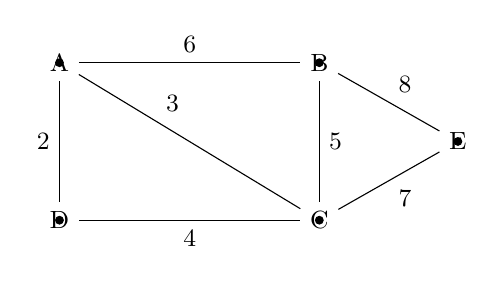
\begin{tikzpicture}[x=1.1cm,y=1.0cm,font=\small]
\node (A) at (0,2) {A}; \node (B) at (3,2) {B}; \node (E) at (4.6,1) {E}; \node (D) at (0,0) {D}; \node (C) at (3,0) {C};
\foreach \p in {A,B,E,D,C}{\fill (\p) circle (1.6pt);}
\draw (A)--node[above]{6}(B); \draw (B)--node[above right]{8}(E); \draw (B)--node[right]{5}(C);
\draw (A)--node[pos=0.35,above right]{3}(C); \draw (A)--node[left]{2}(D); \draw (D)--node[below]{4}(C); \draw (C)--node[below right]{7}(E);
\end{tikzpicture}}\par}{08}{4}{4}
 & b & Define the Harary measure of status. In the given food web, an edge from $X$ to $Y$ means $X$ is food for $Y$. Find the status of each species according to the Harary measure.
\par\vspace{3pt}\centerline{\includegraphics[width=7.5cm]{cs-fig/mm_food.png}}\par & 08 & 3 & 3\\ \hline
\orrow
\qb{8}{a}{Alvin (A) has invited three married couples to his summer house for a week: Bob (B) and Carrie (C) Hanson, David (D) and Edith (E) Irwin, and Frank (F) and Gena (G) Jackson. Since all six guests enjoy playing tennis match against every other guest except his/her spouse. In addition, Alvin is to play a match against each of David, Edith, Frank, and Gena. If no one is to play two matches on the same day, what is a schedule of matches over the smallest number of days.}{08}{4}{4}
 & b & i. Is it possible to have a graph with the degree sequence 1,2,2,3,4,5? If yes, draw an example. If not, give reason.\newline ii. Define the degree of balance of a signed graph. The following graph models the social relation between 4 people with `+' indicating friendship and `$-$' indicating enmity. Find the degree of balance of the graph.
\par\vspace{3pt}\centerline{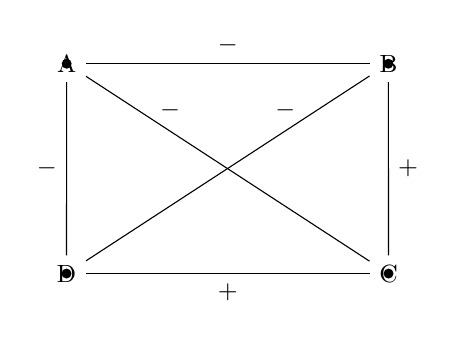
\begin{tikzpicture}[x=1.2cm,y=1.1cm,font=\small]
\node[above left] (A) at (0,2) {A}; \node[above right] (B) at (3,2) {B}; \node[below left] (D) at (0,0) {D}; \node[below right] (C) at (3,0) {C};
\foreach \p in {A,B,C,D}{\fill (\p) circle (1.8pt);}
\draw (A)--node[above]{$-$}(B); \draw (B)--node[right]{$+$}(C); \draw (D)--node[below]{$+$}(C); \draw (A)--node[left]{$-$}(D);
\draw (A)--node[pos=0.25,above right,inner sep=1pt]{$-$}(C); \draw (B)--node[pos=0.25,above left,inner sep=1pt]{$-$}(D);
\end{tikzpicture}}\par & 08 & 3 & 3\\ \hline
\qb{9}{a}{Find the extremals of the functional $\displaystyle\int_{1/10}^{1} y'(1 + x^2 y')\,dx$, if $y\left(\frac{1}{10}\right) = 19$, $y(1) = 1$.}{08}{3}{3}
 & b & A company needs to transport goods from its main warehouse (location A) to its retail outlet (location J). Along the way, the goods must pass through a series of distribution centres (B, C, D, E, F, G, H, I). At each segment of the journey, transport costs are incurred. The company wants to minimize the total transportation cost from A to J. Using dynamic programming, determine the minimum transportation cost from A to J and identify the optimal route. The transportation costs between centres are given in the table below:
\par\vspace{3pt}\centerline{\small\setlength{\tabcolsep}{4pt}\begin{tabular}{c|ccc|}\multicolumn{1}{c}{} & B & C & D\\\cline{2-4} A & 5 & 3 & 6\\\cline{2-4}\end{tabular}\hspace{0.5cm}\begin{tabular}{c|ccc|}\multicolumn{1}{c}{} & E & F & G\\\cline{2-4} B & 4 & 2 & 5\\ C & 3 & 4 & 6\\ D & 5 & 3 & 2\\\cline{2-4}\end{tabular}\hspace{0.5cm}\begin{tabular}{c|cc|}\multicolumn{1}{c}{} & H & I\\\cline{2-3} E & 3 & 4\\ F & 2 & 5\\ G & 6 & 3\\\cline{2-3}\end{tabular}\hspace{0.5cm}\begin{tabular}{c|c|}\multicolumn{1}{c}{} & J\\\cline{2-2} H & 4\\ I & 3\\\cline{2-2}\end{tabular}}\par\nointerlineskip\hbox{} & 08 & 2 & 2\\ \hline
\orrow
\qb{10}{a}{Model the problem of a uniform chain (cable or rope) of length $2l$, suspended under gravity between two points at equal height. Find the curve when the chain is in equilibrium.}{08}{4}{4}
 & b & Discuss any five optimization techniques and any three optimization principles. & 08 & 2 & 2\\ \hline
\end{seeB}
\end{seepaper}

% ---------------- MA266TEU, Model Question Paper (2022 scheme)
\begin{seepaper}
\paperinfo{code={MA266TEU},examline={VI Semester B.E. Examinations -- Model Question Paper},dept={(Institutional Elective)},title={MATHEMATICAL MODELLING},time={03 Hours},maxmarks={100}}
\seehead
\begin{seeinstr}\item Answer all questions from Part A. Part A questions should be answered in first three pages of the answer book only.\item Answer FIVE full questions from Part B.\end{seeinstr}
\seepartA
\begin{seeA}
\qaq{1}{1.1}{The population of California fox are decreasing at the rate of 5\% per year. If their population was 400 in 2013, then how many of them will be left approximately in 2023?}{02}{2}{1}
\qa{1.2}{The growth of an organism follows the law $\dfrac{dx}{dt} = -\dfrac{1}{13}x$. If initially there were 200 of them, then after 13 years, their approximate number will be \blank[1.5cm] and their half-life period is approximately \blank[1.5cm] years.}{02}{2}{3}
\qa{1.3}{In terms of $y_{t+1}$ and $y_{t+2}$, the arbitrary constant $M$ in the equation $y_t = M2^t + N(-3)^t$ is equal to \blank[2cm].}{02}{3}{3}
\qa{1.4}{The curve which extremizes the functional $\displaystyle\int_{10}^{11}\left[y^2 + x^2 y'\right]dx$ is \blank[2cm].}{02}{2}{2}
\qa{1.5}{In the long run, the proportion of time that the given Markov chain will be in state A is \blank[1.5cm] and state B is \blank[1.5cm].
\par\vspace{2pt}\centerline{\begin{tikzpicture}[x=1cm,y=1cm,font=\small,>=Stealth,state/.style={draw,circle,minimum size=0.7cm,inner sep=0pt}]
\node[state] (A) at (0,0) {A}; \node[state] (B) at (3,0) {B};
\draw[->] (B) to[bend right=35] node[above]{0.8} (A);
\draw[->] (A) to[bend right=35] node[below]{0.7} (B);
\draw[->] (A) to[out=150,in=210,looseness=8] node[left]{0.3} (A);
\draw[->] (B) to[out=30,in=-30,looseness=8] node[right]{0.2} (B);
\end{tikzpicture}}\par\vspace{16pt}}{02}{2}{2}
\qa{1.6}{The angle of projection for a projectile to attain\newline a) the maximum horizontal distance should be \blank[1.5cm].\newline b) the maximum height should be \blank[1.5cm].}{02}{1}{3}
\qa{1.7}{In the following figure, with respect to dynamic programming, the value of $f_1^*(O)$ is \blank[1.5cm].
\par\vspace{3pt}\centerline{\begin{tikzpicture}[x=1.15cm,y=0.95cm,font=\small,>=Stealth]
\tikzset{b/.style={draw,minimum size=0.5cm,inner sep=1pt}}
\node[b] (O) at (0,0) {O}; \node[b] (A) at (1.8,1.3) {A}; \node[b] (B) at (3.6,1.3) {B};
\node[b] (S) at (1.8,0) {S}; \node[b] (D) at (5.4,0) {D};
\node[b] (R) at (1.8,-1.3) {R}; \node[b] (U) at (3.6,-1.3) {U};
\draw[->] (O)--node[above left]{6}(A); \draw[->] (A)--node[above]{6}(B); \draw[->] (B)--node[above right]{8}(D);
\draw[->] (O)--node[above]{5}(S); \draw[->] (S)--node[pos=0.3,right]{3}(B); \draw[->] (S)--node[above]{7}(D);
\draw[->] (S)--node[pos=0.3,right]{1}(U); \draw[->] (O)--node[below left]{4}(R);
\draw[->] (R)--node[below]{1}(U); \draw[->] (U)--node[below right]{2}(D);
\end{tikzpicture}}\par\vspace{2pt}}{02}{2}{4}
\qa{1.8}{Write the linear equations associated with the following signal-flow graph:
\par\vspace{3pt}\centerline{\includegraphics[width=4.6cm]{cs-fig/mmq_sfg.png}}\par\nointerlineskip\hbox{}}{02}{2}{4}
\qa{1.9}{Given the initial state vector $(1, 0)$ and the transition matrix shown below, find the state vector corresponding to two steps later ($n = 2$). $\begin{bmatrix}0.13 & 0.87\\ 0.91 & 0.09\end{bmatrix}$}{02}{1}{1}
\qa{1.10}{`Edge coloring' is the assigning of colors to the edges so that no two adjacent edges have same color. Consider a simple connected graph $G$ in which the number of vertices is equal to the number of edges, and every vertex has degree 2. What is the minimum number of colors required to `edge-color' $G$?}{02}{1}{2}
\end{seeA}
\seepart{PART-B}
\begin{seeB}
\qb{2}{a}{Give a note on the classification of mathematical models giving at least four examples.}{08}{1}{1}
 & b & Drug is induced in a patient's bloodstream at regular intervals of duration $T$ each. Simultaneously the drug disappears at a rate proportional to the concentration $c(t)$ of the drug present at any time $t$. Determine the differential equation governing $c(t)$, solve it and interpret the results. & 08 & 3 & 3\\ \hline
\qb{3}{a}{Mathematically establish the Hardy-Weinberg law in genetics.}{08}{3}{2}
 & b & A person takes a loan of \rupee $S_0$ with $i$ as the compound interest rate per month. If the loan is to be paid back in $n$ equal instalments by paying \rupee $R$ per month, then show that $R = S_0\dfrac{i}{1-(1+i)^{-n}}$. & 08 & 2 & 2\\ \hline
\orrow
\qb{4}{a}{Bring out the dynamics of price and quantity of a commodity produced by a farm according to the Cobweb model.}{08}{3}{2}
 & b & i. Solve the difference equation $x_{t+2} = 4(x_{t+1} - x_t)$, $t \ge 0$, $x_0 = 1$, $x_1 = 3$.\newline ii. The number of virus affected files in a system is 5000 (to start with) and this increases 200\% every two hours. Model this using a difference equation and find the number of virus affected files in the system after one day. & 08 & 2 & 2\\ \hline
\qb{5}{a}{Check if the transition probability matrix $\begin{bmatrix}0 & 1 & 0\\ 0 & 0 & 1\\ 1/3 & 1/3 & 1/3\end{bmatrix}$ is irreducible. Also find its stationary probability vector.}{08}{2}{1}
 & b & A city is served by two cable TV companies, Best TV and Cable Cast. Due to their aggressive sales tactics, each year 40\% of Best TV customers switch to Cable Cast. On the other hand, 30\% of the Cable Cast customers switch to Best TV. If the initial market share for Best TV is 20\% and for Cable Cast is 80\%, find the market share of each company after 5 years. & 08 & 2 & 3\\ \hline
\orrow
\qb{6}{a}{Consider a network containing five individuals viz.\ $a, b, c, d$ and $e$. The system $a$ can communicate to only $b$ and $c$ and its chances of communicating with each are in the ratio 3:2 respectively. Similarly, $b$ communicates with $a$ and $c$ in ratio 1:1; $c$ can communicate with $a, b$ and $d$ in ratio 4:3:3; $d$ communicates with $c$ and $e$ in ratio 3:7 and $e$ can communicate to $b$ only. Model the situation as a Markov chain and rank the five individuals in accordance with their importance in the network in the long run.}{08}{2}{1}
 & b & A gambler has \rupee 2. He bets \rupee 1 at a time and wins \rupee 1 with probability $\frac{1}{2}$. He stops playing if he ends up with no money or wins \rupee 4.\newline a. What is the TPM of the related Markov chain?\newline b. What is the probability that he has lost his money at the end of 5 plays?\newline What is the probability that the game lasts more than 7 plays? & 08 & 3 & 3\\ \hline
\qb{7}{a}{At the end of the school day, all the students plan on driving from school (vertex A) to the concert (at vertex Z). The edges in the graph below represent one-way roads, and the weight of each edge represents the number of vehicles (in hundreds) that particular road can handle in one hour. What is the greatest number of vehicles that can get from school to the concert in one hour? How many vehicles should take each road?
\par\vspace{3pt}\centerline{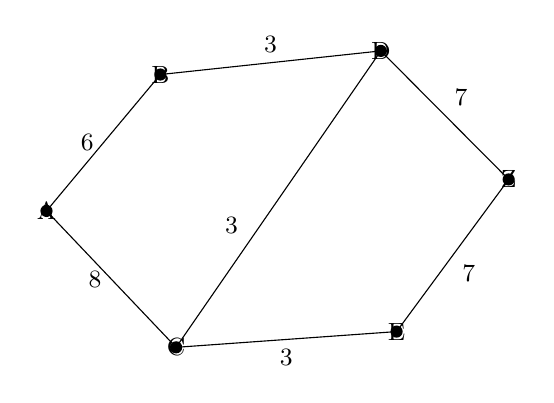
\begin{tikzpicture}[x=1.0cm,y=1.0cm,font=\small]
\node[left] (A) at (0,0) {A}; \node[above] (B) at (1.2,1.5) {B}; \node[above] (D) at (4.0,1.8) {D}; \node[right] (Z) at (5.4,0.4) {Z};
\node[below] (E) at (4.2,-1.3) {E}; \node[below] (C) at (1.4,-1.5) {C};
\foreach \p in {A,B,D,Z,E,C}{\fill (\p.center) circle (2.2pt);}
\draw (A.center)--node[left]{6}(B.center); \draw (B.center)--node[above]{3}(D.center); \draw (D.center)--node[above right]{7}(Z.center);
\draw (A.center)--node[left]{8}(C.center); \draw (C.center)--node[below]{3}(E.center); \draw (E.center)--node[below right]{7}(Z.center);
\draw (C.center)--node[pos=0.35,above left]{3}(D.center);
\end{tikzpicture}}\par\nointerlineskip\hbox{}}{08}{2}{4}
 & b & i. Basavaraj has picked 8 friends for a project team such that they are all friends among themselves. Considering A and B being friends as a single friendship, is it possible that there are totally 38 friendships? Substantiate your answer.\newline ii. Define the degree of balance of a signed graph. The following graph models the social relation between 4 people with `+' indicating friendship and `$-$' indicating enmity. Find the degree of balance of the graph.
\par\vspace{3pt}\centerline{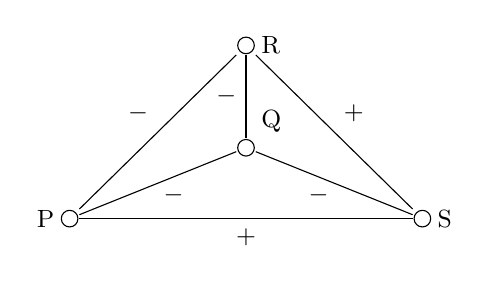
\begin{tikzpicture}[x=1.4cm,y=1.0cm,font=\small]
\node (R) at (1.6,2.2) {}; \node (Q) at (1.6,0.9) {}; \node (P) at (0,0) {}; \node (S) at (3.2,0) {};
\foreach \p/\l/\a in {R/R/right,Q/Q/above right,P/P/left,S/S/right}{\draw[fill=white] (\p) circle (3pt) node[\a=2pt]{\l};}
\draw (P)--node[above left]{$-$}(R); \draw (R)--node[left]{$-$}(Q); \draw (R)--node[above right]{$+$}(S);
\draw (P)--node[below,pos=0.6]{$-$}(Q); \draw (Q)--node[below,pos=0.4]{$-$}(S); \draw (P)--node[below]{$+$}(S);
\end{tikzpicture}}\par\nointerlineskip\hbox{} & 08 & 3 & 4\\ \hline
\orrow
\qb{8}{a}{The Fig 8b shows an intersection of two streets where there is often heavy traffic. There are seven traffic lanes $L1, L2, \dots L7$ where vehicles can enter the intersection of these two streets. A traffic light is located at this intersection. During a certain phase of this traffic light, those cars in lanes for which the light is green may proceed safely through the intersection. Model this situation by a graph giving out the details as to what the vertices and the edges represent. Use that graph to determine whether it is possible with four phases, for cars in all lanes to proceed safely through the intersection.
\par\vspace{3pt}\centerline{\includegraphics[width=5.4cm]{cs-fig/mmq_fig8b.png}}\par\centerline{\small Fig 8b}\par\nointerlineskip\hbox{}}{08}{2}{4}
 & b & Define the Harary measure of status. Find the Harary measure of each individual in the organizational graph shown in Fig 9c.
\par\vspace{3pt}\centerline{\begin{tikzpicture}[x=0.9cm,y=0.9cm,font=\small,>=Stealth]
\node[circle,draw,inner sep=1.5pt,label=above:$a$] (a) at (0,0) {}; \node[circle,draw,inner sep=1.5pt,label=right:$g$] (g) at (2,0) {};
\node[circle,draw,inner sep=1.5pt,label=left:$b$] (b) at (-1.2,-1.8) {}; \node[circle,draw,inner sep=1.5pt,label=above right:$c$] (c) at (1.0,-1.8) {};
\node[circle,draw,inner sep=1.5pt,label=right:$h$] (h) at (2.6,-1.8) {}; \node[circle,draw,inner sep=1.5pt,label=right:$i$] (i) at (1.8,-3.4) {};
\node[circle,draw,inner sep=1.5pt,label=left:$d$] (d) at (-1.2,-3.4) {}; \node[circle,draw,inner sep=1.5pt,label=below:$e$] (e) at (-2.2,-5.0) {}; \node[circle,draw,inner sep=1.5pt,label=below:$f$] (f) at (-0.3,-5.0) {};
\draw[->] (a)--(g); \draw[->] (a)--(b); \draw[->] (a)--(c); \draw[->] (b)--(d); \draw[->] (c)--(h); \draw[->] (c)--(i); \draw[->] (h)--(i); \draw[->] (c)--(f); \draw[->] (d)--(e); \draw[->] (d)--(f);
\end{tikzpicture}}\par\centerline{\small Fig 9c}\par\nointerlineskip\hbox{} & 08 & 3 & 4\\ \hline
\qb{9}{a}{A person decides to travel from a place A to a place J. The journey would require traveling by a stagecoach through different cities on the paths of which there is danger of attack by thieves. Life insurance policies were offered to the passengers, the safest route would be the one with the cheapest total life insurance policy. The details of the insurance from one place to another are given below. Model it through a directed graph and find the route which minimizes the cost using dynamic programming.
\par\vspace{3pt}\centerline{\small\setlength{\tabcolsep}{4pt}\begin{tabular}{c|ccc|}\multicolumn{1}{c}{} & B & C & D\\\cline{2-4} A & 1 & 3 & 6\\\cline{2-4}\end{tabular}\hspace{0.5cm}\begin{tabular}{c|ccc|}\multicolumn{1}{c}{} & E & F & G\\\cline{2-4} B & 5 & 4 & 6\\ C & 4 & 3 & 2\\ D & 1 & 4 & 5\\\cline{2-4}\end{tabular}\hspace{0.5cm}\begin{tabular}{c|cc|}\multicolumn{1}{c}{} & H & I\\\cline{2-3} E & 5 & 2\\ F & 3 & 6\\ G & 3 & 3\\\cline{2-3}\end{tabular}\hspace{0.5cm}\begin{tabular}{c|c|}\multicolumn{1}{c}{} & J\\\cline{2-2} H & 5\\ I & 2\\\cline{2-2}\end{tabular}}\par\nointerlineskip\hbox{}}{08}{1}{2}
 & b & Model the problem of light passing from a point A to a point B as a variational problem by applying Fermat's principle of least time. Show that a consequence of this modelling is the Snell's law of refraction. & 08 & 3 & 4\\ \hline
\orrow
\qb{10}{a}{Discuss any five optimization techniques and any three optimization principles.}{08}{1}{2}
 & b & A particle descends from one point to another point in the absence of friction under the action of gravity. Model the situation as a variational problem so as to find the path of the quickest descent. & 08 & 3 & 4\\ \hline
\end{seeB}
\end{seepaper}

\end{document}
